\section{Related Work and Industrial Applications}
	\label{sec:related_work}
	As an active research area, there is a great wealth of work solely focused on the optimisation of the placement of nodes as well as mesh networks, wireless or otherwise. Considering the hardware involved, the deployment of a wireless mesh network must consider the strength and configuration of the radios, its resistance to the elements of the environment it is placed in, the source of the power and its reliability as well as that level of reliability's effect on the choice on how data is stored. Depending on the requirements of the network, legal requirements might add further constraints such as a given amount of time logs and records must be kept for and the ability to verify the authenticity and accuracy \cite{gdpr} of those logs.

	This section details the various areas related to wireless mesh networks and the optimisation of their placement, both traditional and more novel approaches, including work done by other researchers with similar but distinct objectives. We also discuss the various ways in which industry might seek to apply these concepts.

	\subsection{Distributed Systems}
		\label{sec:related_work_distributed} 
		When we turn to the software involved we can observe that mesh networks are an example of distributed systems, another very active research area looking to tackle problems of distributed consensus \cite{lamport2019byzantine} \cite{paxos} \cite{raft}, node failure and parallel algorithms to name just a few. Each of these problems are difficult and solutions inherently involve some trade-off that must be made in line with the constraints and desired properties of the solution.

	\subsection{Extraplanetary Applications}
		\label{sec:related_work_spacex} 
		As covered in the introduction, wireless mesh networks are deeply flexible and have a wide number of possible applications\cite{akyildiza47wireless}. A very recent example of this is SpaceX's Starlink project which seeks to deploy 2,825 satellites. In addition to each of the satellites covering an individual area to provide a single intermediary between a user and a "gateway earth station" for satellite internet access, "The system will also employ optical inter-satellite links for seamless network management and continuity of service\cite{fccspacextechnicala}." Contained in this one sentence is a world of complexity with regards to implementation that takes advantage of cutting edge hardware and software research with heavy use of the research into areas such as distributed systems and radio equipment. As you may be able to guess from figure \ref{fig:spacex}, the placement of these nodes changes from moment to moment as the satellites orbit earth according to expected traffic.
		\begin{figure}[H]
		\centering
		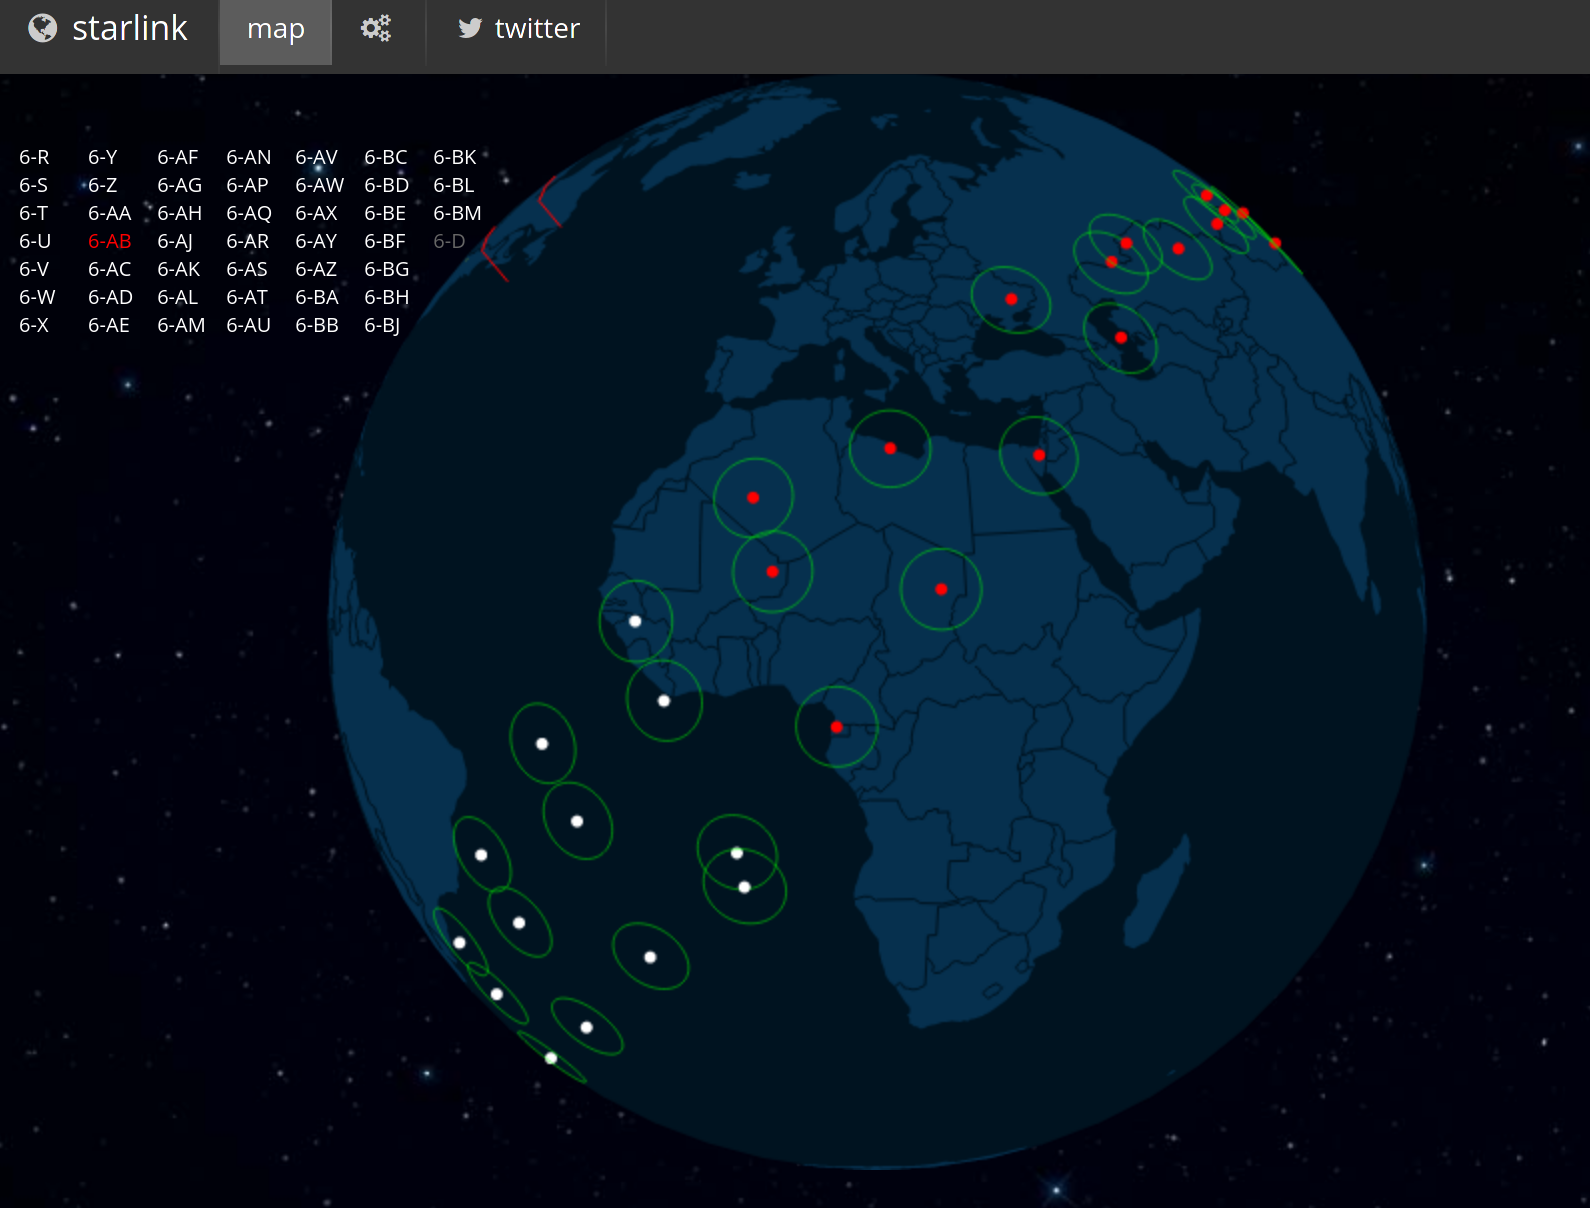
\includegraphics[scale=0.21]{graphics/spacex_map}
		\caption{SpaceX Starlink Satellite Map \cite{satellitemap}}
		\label{fig:spacex}
		\end{figure}
		
	\subsection{Optimisation}  
		\label{sec:related_work_optimisation} 
		Focusing solely on the subject of node placement in wireless mesh networks, there has been so much research that a survey of some of the many strategies and techniques in node placement exists\cite{younis2020placementsurvey}. This survey goes into detail concerning node distribution, deployment objectives, dynamic repositioning of nodes and existing open research problems. The impact of the desired properties such as primary objectives and constraints of the system on node placement is repeatedly highlighted and given its own column on multiple tables, making it clear that there is no `one size fits all' approach to node placement. 

		From this we can infer that if we wish to build software that evaluates the suitability of and optimises node placements in a generic way it is of vital importance that we allow for users of that software to provide their own constraints and objectives comprehensively. While there is a place for novice users with no ability to program making use of GUI software, utilising complex optimisation software will require the users to be programmers capable of providing functions to the library that we have developed in order for the software to accurately evaluate the suitability of a set of node placements according to their unique specifications.

		\subsubsection{Traditional Algorithms}
			\label{sec:related_work_traditional}
			Sharpening our focus still onto the optimisation of node placement we find a few common optimisations. The first one is random node distribution, which is covered in the aforementioned survey.\cite{younis2020placementsurvey} Many research papers already exist that have considered the use of random node distribution and evaluation\cite{wang2010coverage} according to given constraints and objectives. However some researchers go further than this naive optimisation approach, considering single and multi-objective genetic algorithms (MOGAs)\cite{zhang2017flexible}, greedy algorithms and cluster placement for enhanced performance\cite{bi2015node}. An important consideration is that MOGAs are more suited for `objective' functions with fast execution times, but not for those that are slow to compute. This is because genetic algorithms typically create a population of candidate solutions\cite{banzhaf1998genetic} the size of which is dependent on the nature of the problem but could well be in the thousands. As such, evaluating each of the population for an expensive algorithm for each generation quickly becomes computationally infeasible.

		\subsubsection{Bayesian Optimisation} 
			\label{sec:related_work_bayesian} 
			Bayesian optimisation is an approach to global optimisation that evaluates data as it is collected using a `sequential' design strategy\cite{movckus1975bayesian}. This strategy makes Bayesian optimisation uniquely suited to optimising computationally expensive `cost' functions,\cite{brochu2010tutorial} which are functions that take a range of values and return some real number, allowing that result to be compared with other results of other ranges of values. This methodology makes no assumption about the form or behaviour of the function, treating it as a `black box'.

			As of writing, we have not seen any evidence that the approach of Bayesian optimisation has been used or published and as such this research is novel in this way. Shahriari et al. discuss Bayesian optimisation at length in `Taking the Human Out of the Loop: A Review of Bayesian Optimization'\cite{shahriari2015taking}, laying out many of the possible and already existing applications of Bayesian optimisation as well as thorough psuedo-code implementations of a number of ways in which Bayesian optimisation can be implemented. `Acquisition' functions are also discussed which are used to find the exact query points that will best further guide the algorithm's understanding of the search space. More detail about Bayesian optimisation is given in chapter \ref{sec:bayesian}.
			\begin{figure}[H]
			\centering
			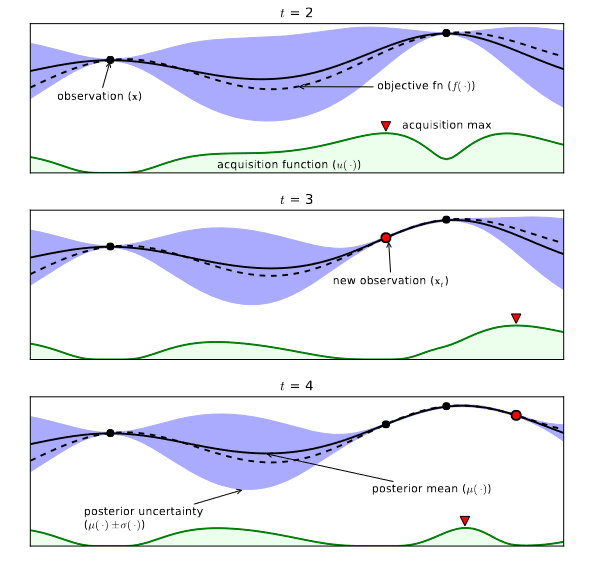
\includegraphics[scale=0.6]{graphics/bayesian_1d}
			\caption{Bayesian Optimisation on a toy one-dimensional problem. \cite{brochu2010tutorial}}
			\label{fig:bayesian_1d}
			\end{figure}
	\subsection{Industrial Applications}
		\label{sec:related_industrial}
		As we've discussed in section \ref{sec:problem_broadness}, there are a wide range of places industry might seek to apply the optimisation of wireless node placement. Internet-of-things devices are increasingly common in consumer and office environments \cite{evans2011internet}, all of these devices sharing the key characteristic of requiring strong and reliable access to a network in order to exchange information among each other and often with the outside world. Poor signal inhibits the advantages of these devices and so maximising signal ($\approx$ minimising distance) is of vital importance.

		In the example of Starlink, running network simulations and experiments long before the launch of the network will surely have taken place to plan traffic flows and measure the strength of the connection from the surface to satellites and satellite to satellite. The expense involved in launching such a network would preclude testing in a live environment. The placement of individual satellites would also heavily benefit from the optimisation of placement according to the required bandwidth at certain points in the day.

		On a different scale, office employees are increasingly using wireless devices instead of wired computers at fixed desks. Under these circumstances having strong connection coverage is important to ensure that employees attempting to access local and remote resources can do so efficiently. Planning the placement of nodes to optimise for coverage would be wise and not doing so would have a negative impact on employees.